\chapter{Pipeline security}
\section{Introduction}
Pipeline security can be considered to be a large part of the process of securing software development, from its source code to production deployment. The group has categorized pipeline security into two aspects - security in the pipeline and security of the pipeline. In many ways implementing both security in the pipeline and of the pipeline will increase the overall security of the pipeline. Below the group will look closer into what are important security measures within these two. 
\\~\\
Below is a figure of a \gls{Pipeline} without any security measures implemented. As the different measures are presented in the following chapter, they will be added to the pipeline. In the end, this will result in a complete, secure pipeline.

\vspace{2mm}
\begin{figure}[H]
    \centering
    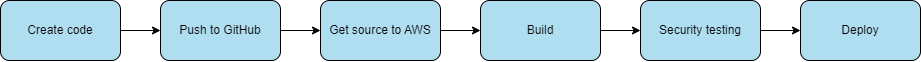
\includegraphics[width=0.8\columnwidth]{Images/SecurePipeline-Page-3.drawio.png}
    \caption{Pipeline without any security measures}
    \label{fig: Pipeline without any security measures}
\end{figure}
\section{Security in the pipeline}
Security in the pipeline is the process of implementing different measures and controls to protect the code that is being sent through the pipeline from various security threats. The pipeline commonly consists of multiple phases like code development, testing, and deployment, all of which may be susceptible to various security threats, like unauthorized access, data breaches, malware, and denial-of-service attacks. Security in the pipeline is crucial to secure the integrity and confidentiality of software applications and data.

\subsection{Code Scanning}
%du tester koden som skal bli deployet, alstå det som ligger inni pipelinen. Sjekkes for sårbarheter etc
Code scanning is a security measure where code is analyzed with the help of a tool to find security vulnerabilities and coding errors. Code scanning serves as a preventive measure against developers introducing new issues. During this step, you can perform a SAST scan using specialized tools that are designed to scan through code. 
\\
\\
GitHub provides an integrated code scanner called CodeQL. CodeQL extracts all source code into a relational database optimized for CodeQL analysis.  It can then be queried to identify insecure patterns in the code and other vulnerabilities. The user can take advantage of a large number of queries already made by other developers, or they can make their own. An example of a simple query could be getting the location of all method calls in the code. 
 \cite{codeql}

 \vspace{2mm}
\begin{figure}[H]
    \centering
    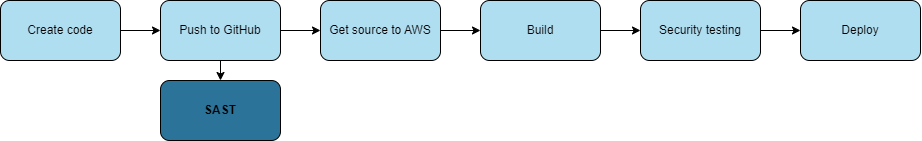
\includegraphics[width=0.8\columnwidth]{Images/pipeline2.png}
    \caption{Pipeline with implemented SAST scan}
    \label{fig: Pipeline with implemented SAST scan}
\end{figure}

\subsection{Scan Dependencies and Open Source Libraries}
All dependencies, open-source libraries, and third-party \gls{artifact}s that have been utilized should be validated. This can be done by comparing their checksum against a reliable, good source and validating any cryptographic signatures. If any third-party software was implemented in the application it's important to conduct an \acrshort{sca} scan using suitable tools to identify whether any vulnerable open-source software was used. \cite{bestpracticeSupplyChain}

\vspace{2mm}
\begin{figure}[H]
    \centering
    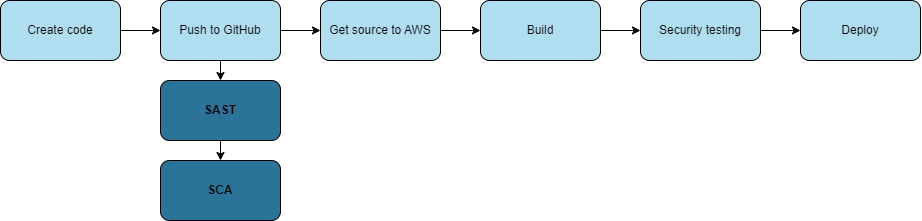
\includegraphics[width=0.8\columnwidth]{Images/pipeline3.png}
    \caption{Pipeline with implemented SCA scan}
    \label{fig: Pipeline with implemented SCA scan}
\end{figure}

\subsection{Secret Scanning}
To prevent or identify accidental exposure of "secrets", like access tokens, SSH keys, or other credentials, one should execute a secret scanning on a Git repository. Secret scanning tools, such as GitHub's secret scanning, can be used to find these vulnerabilities, and alert developers to potential security risks. \cite{GithubSecretScanning}

\vspace{2mm}
\begin{figure}[H]
    \centering
    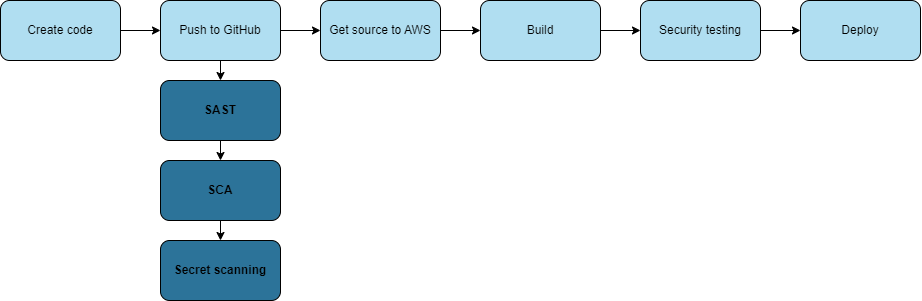
\includegraphics[width=0.8\columnwidth]{Images/pipeline4.png}
    \caption{Pipeline with implemented secret scan}
    \label{fig: Pipeline with implemented secret scan}
\end{figure}

\subsection{Dynamic scanning}
In software best practices, it is recommended to run multiple tests and scans to identify bugs and errors - where one of these tests is \acrlong{dast} (\acrshort{dast}).\cite{bestpracticeSupplyChain} This scanning method tries to penetrate the application, attempting to identify vulnerabilities and weaknesses in it. One can implement a tool specialized for DAST scans, such as OWASP Zap, which can identify security risks like \gls{Cross-site scripting}, \gls{SQL-injection} or path traversal.\cite{dynamictesting}


\subsubsection{The Limitations of DAST Tools}
Even though \acrshort{dast} can be used to identify potential vulnerabilities, certain types of threats may go undetected. For this reason, the company should engage a red team, which is a group of experts capable of performing penetration testing. A pen test will provide a more realistic test, as it simulates a real-world attack, detects more complex vulnerabilities, and provide a more comprehensive view of an application's security posture. A pen test can also function as a validation of the \acrshort{dast} scan, as it can help determine if the vulnerability can be exploited and the potential impact of the vulnerability. \cite{dastpentesting}

\vspace{2mm}
\begin{figure}[H]
    \centering
    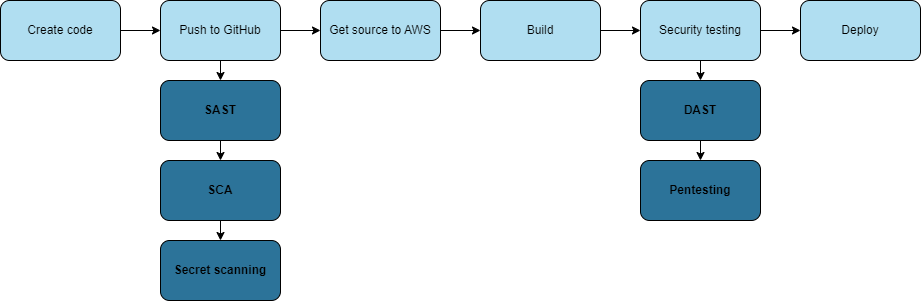
\includegraphics[width=0.8\columnwidth]{Images/pipeline5.png}
    \caption{Pipeline with implemented DAST scan and pentesting}
    \label{fig: Pipeline with implemented DAST scan and pentesting}
\end{figure}

\subsection{Artifacts}




\section{Security of the pipeline}
\label{Security of the pipeline}
Security of the pipeline refers to the measures taken to protect the pipeline and the underlying infrastructure and network involved in processing the code that passes through it. To ensure the pipeline's security, it is limited to performing its intended functions and stops unauthorized access to restricted resources.

\subsection{Branch Protection}
Branch protection ensures that specific criteria are met before code can be merged \cite{branch}. This feature allows users to create branch protection rules that enforce specific workflows for one or multiple branches, such as mandating an approving review or passing status checks for all pull requests merged into the protected branch. Access to this feature of GitHub is available for all users.
\\
Enforcing branch protection makes introducing errors and vulnerabilities into the secured branch less likely. In addition, branch protection creates a more precise development process by providing guidelines and requirements for making changes in the code. This helps ensure that all team members are aligned towards the same goal and working together effectively.  


\vspace{2mm}
\begin{figure}[H]
    \centering
    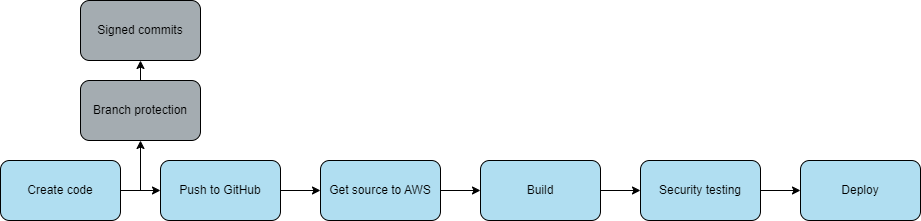
\includegraphics[width=0.8\columnwidth]{Images/pipeline6.png}
    \caption{Pipeline with implemented branch protection rules}
    \label{fig: Pipeline with implemented branch protection rules}
\end{figure}

subsection{Access Control}
Access control is crucial to regulating individuals' access to specific resources such as GitHub \cite{accesscontroll}. It involves implementing measures to determine the appropriate level of access for each individual while following the "least privilege" principle. As specified by \acrshort{nist} \cite{leastprivilege}, this principle entails designing a security architecture so that each entity is granted only the minimum system resources and authorizations needed to perform its function. 

In GitHub, permission controls access, which refers to the capability to execute specific tasks. Furthermore, team members can have specific roles assigned to them, and certain permissions can be granted to both individuals and groups. By following these measures, organizations can effectively manage access control and reduce risks associated with unauthorized access to critical resources. 
\\~\\
Secure authentication is a crucial aspect of maintaining system security. It involves implementing measures to ensure that only authorized users can access a system and that their access is limited to the specific resources needed to perform their duties.
\\~\\
Organizations can bolster their authentication process by implementing conditional access protocols. By specifying specific rules and conditions, the system can determine the appropriate times, locations, and methods for users to gain access. For example, an organization might require multi-factor authentication for all users accessing the system outside the corporate network. In addition, they might limit access to specific applications or data based on the user's role or location.
\\~\\
Conditional access is a critical component of a comprehensive security strategy for organizations. It enables effective control of system access, reducing the risk of unauthorized access or data breaches and ensuring compliance with regulatory requirements. This access control should be implemented across all system components and at every stage in the pipeline to provide maximum protection. Therefore, it is essential to practice access control diligently and consistently.

Access control should be done before the code enters any software, in this case, GitHub and \acrshort{aws}, to ensure access regulation at any time, as shown in Figure \ref{fig: Pipeline with implemented access control}.

\vspace{2mm}
\begin{figure}[H]
    \centering
    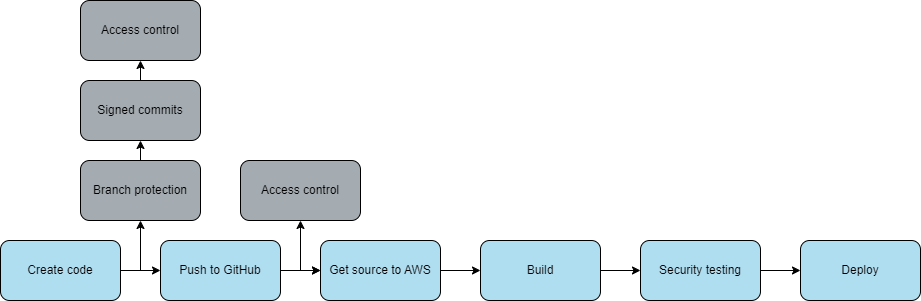
\includegraphics[width=0.8\columnwidth]{Images/pipeline7.png}
    \caption{Pipeline with implemented access control}
    \label{fig: Pipeline with implemented access control}
\end{figure}
 
\subsection{File Storage and Preservation}
Proper pipeline security requires significant attention to file storage and preservation. File storage and preservation help secure the pipeline over time by doing regular backups of the data related to the pipeline. In addition, maintaining redundant copies of critical data can minimize the risk of data loss due to attacks or other security breaches. 
\\~\\
Another important aspect of file storage and preservation is access control, which should be restricted so that individuals only have the necessary access. As a result, this can minimize the chances of data tampering or data theft.

\section{Security in maintenance}
Once the deployment process is complete, the application is transferred to the cloud environment in \acrlong{aws} \cite{awsafterdep}. It is essential at this stage to keep the security up to date to ensure that the application and data are protected. AWS offers a range of best practices organizations can follow to decrease risks associated with cloud computing and ensure that the  \acrshort{aws} environment is secure 
\\~\\
After successful deployment, ensuring the infrastructure is secure and optimized for performance is essential. In addition, regular maintenance and updates are necessary to solve security issues and add new features to the system. It is also essential to perform regular backups and disaster recovery testing to protect the data and applications. Staying up-to-date with maintenance and testing can minimize downtime and improve system reliability. 
\\~\\
Continuous monitoring of cloud-based applications is crucial to detect any issues or potential threats. This encompasses identifying errors, performance issues, security vulnerabilities, and other related concerns. \acrshort{aws} offers specialized tools for this type of monitoring, like AWS Cloudtrail\footnote{Available at: \url{https://aws.amazon.com/cloudtrail/}} and AWS X-ray\footnote{Available at: \url{https://aws.amazon.com/xray/}}. 
\\~\\
Various security tests, such as security scans and penetration testing, should be performed during the development phases to identify potential vulnerabilities and address them before deployment. However, it is also essential to continue testing after the deployment to ensure that any new vulnerabilities are identified and addressed as soon as possible. Regular security scans and penetration testing can significantly reduce the risk of exploitation. By conducting these tests regularly, the organization can keep track of any possible security problems and take proactive measures to mitigate them.
\\~\\
As a protective measure, the organization should set up a web application firewall like AWS WAF\footnote{Available at \url{https://aws.amazon.com/waf/}}, to prevent malicious application attacks such as \gls{SQL-injection}, \gls{Cross-site scripting} and other attacks. AWS's WAF service offers a managed set of protective rules, allowing customized rules and access control lists based on the company's needs and risk models. This makes it possible to provide web application security with more customization and specificity. Securing an application against \gls{ddos} is an important additional step. AWS Shield\footnote{Available at \url{https://aws.amazon.com/shield/}} is a service that an organization can utilize to achieve this. 
\\~\\
Maintaining security is crucial during the maintenance phase of the SDLC, which starts after the application has been deployed. It is critical to keep up with regular maintenance and testing during this phase and take proactive measures to mitigate any issues that may arise. Organizations can identify and address potential security vulnerabilities beforehand to prevent them from becoming significant issues. This is particularly crucial when deploying applications to the cloud due to the complex and ever-changing security environment. Best practices such as regular security audits, vulnerability scans, and patches can ensure the application remains secure and protected against potential threats. Monitoring for unusual or suspicious activity can also aid in detecting and preventing security breaches. Organizations can help ensure their AWS applications' continued reliability and security by prioritizing security throughout the maintenance phase.


\section{Finished pipeline}
Figure \ref{fig: Pipeline with all security measures implemented} illustrates a finished pipeline after all security measures are included. This also includes maintenance.  

\vspace{2mm}
\begin{figure}[H]
    \centering
    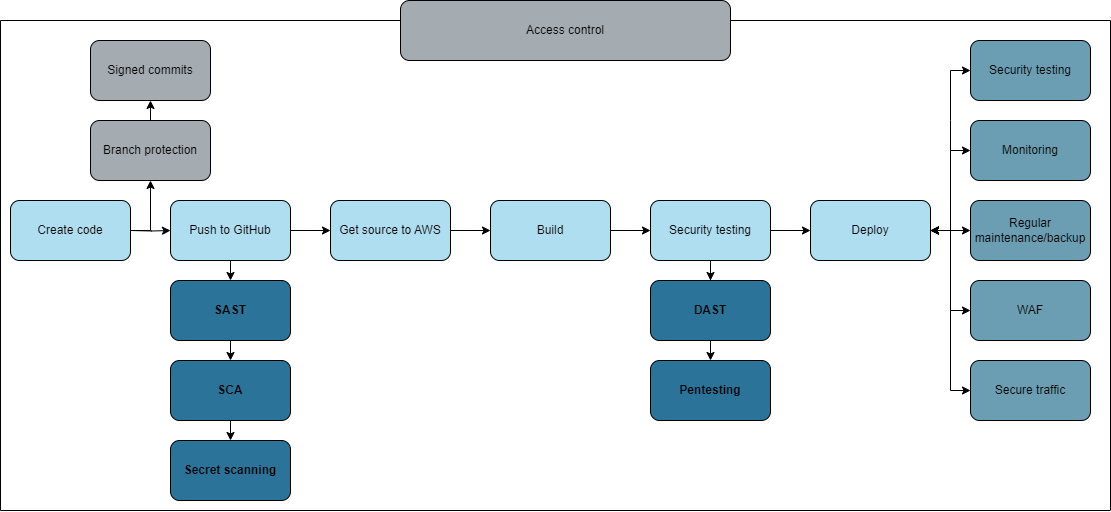
\includegraphics[width=0.8\columnwidth]{Images/FinalPipeline.png}
    \caption{Pipeline with all security measures implemented}
    \label{fig: Pipeline with all security measures implemented}
\end{figure}




\section{Framework}
\subsection{Introduction}


\subsection{Supply-chain Levels for Software Artifacts}
\acrlong{slsa}\footnote{Available at: https://slsa.dev/} is a framework for securing the software supply chain created by Google in collaboration with OpenSSF\footnote{Available at: https://openssf.org/}. The framework is made into a common vocabulary checklist for developers to evaluate the security of the software they are creating. \acrshort{slsa} is organized into tracks and levels. The levels refer to the increasing security guarantee of the supply chain, the highest level being level 3. The levels are split further into tracks. Tracks are certain aspects of the supply chain, for example, the Build track, which currently is \acrshort{slsa}s only track. \cite{SLSAgeneral}

\vspace{2mm}
\begin{figure}[H]
    \centering
    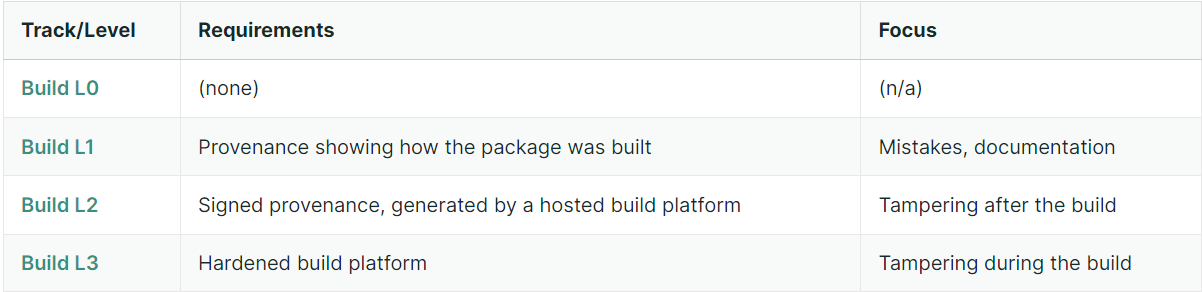
\includegraphics[width=0.8\columnwidth]{Images/slsalevels.png}
    \caption{SLSA levels for the Build track} Adapted from: \cite{SLSAlevels}
    \label{fig: SLSA levels for the Build track}
\end{figure}

Currently, there are three levels split into one track. To achieve the different build levels, the developers have to do the following:
\\~\\
To achieve \acrshort{slsa} Build Level 1, the developers are required to use a consistent build process, which can easily be adopted. Additionally, the build platform has to generate \gls{provenance} automatically, which describes how the artifact was built. This includes information on the entity responsible for building the package, the specific build process used, and the top-level inputs utilized during the build process.
\\~\\
To achieve \acrshort{slsa} Level 2, all Level 1 requirements must be in place. Further, the build has to be run on a platform that generates signs the \gls{provenance}. This \gls{provenance}'s authenticity also has to be verified.
\\~\\
Similarly to Level 2, all previous level requirements have to be achieved to get to \acrshort{slsa} Level 3. In addition, the build platform has to have controls to secure the secrets used for signing \gls{provenance}and prevent runs from the same project impact each other. 


\subsection{Secure Software Development Framework}
\acrlong{ssdf}\footnote{Latest version: https://nvlpubs.nist.gov/nistpubs/SpecialPublications/NIST.SP.800-218.pdf} is a framework consisting of practices for a secure software development, created by \acrlong{nist}. The company should integrate the \acrshort{ssdf} into their already existing software development practices. SSDF does not specify how each practice should be implemented. It emphasizes the outcome of the practices rather than how to perform them. Organizations in any sector or community can use the SSDF, regardless of their size or level of cybersecurity competence. This framework is intended to be user-friendly and adaptable, making it appropriate for a wide range of businesses with varied levels of cybersecurity knowledge. Organizations can use the SSDF to adopt secure software development practices and reduce the risk of potential security vulnerabilities. The framework does not introduce new practices or define new terminology, but it rather presents a set of high-level practices that are based on known standards, guidelines, and documents relevant to secure software development practices. 

The benefits of describing the practices at a high level include that they can be used by organizations in every industry and community, despite their size or level of cybersecurity knowledge. It can also help companies that buy and use software to understand the secure software development methods used by the suppliers they work with. 

The practices are separated into four groups:
\begin{itemize}
  \item Prepare the Organization (PO)
  \item Protect the Software (PS)
  \item Produce Well-Secured Software (PW)
  \item Respond to Vulnerabilities (RV)
\end{itemize}

Each practice definition has the following components:
\begin{itemize}
  \item Practice
  \item Task
  \item Notional Implementation Examples
  \item References
\end{itemize}






